\documentclass[11pt]{article}
\usepackage[margin=1in]{geometry}
\usepackage{booktabs}
\usepackage{tikz}
\usetikzlibrary{arrows.meta,positioning,shapes.geometric,fit}
\usepackage{setspace}
\setstretch{1.1}

\title{Final Project Report: Multimodal Ad Impact Prediction}
\author{NeuroBioSense DL Project}
\date{}

\begin{document}
\maketitle

\section*{1. Problem Statement}
This project predicts advertisement impact while users are watching videos. The target is binary valence:
negative vs positive response.

\section*{2. Dataset and Label Strategy}
\begin{itemize}
    \item Video modality: advertisement clips and facial dynamics.
    \item Physiological modality: 32-Hz signals (BVP, EDA, TEMP, ACC X/Y/Z).
    \item Binary valence mapping: Positive = Joy/Surprise, Negative = Sadness/Anger/Disgust/Fear.
    \item Neutral class excluded for binary setting.
    \item Participant-level split is applied to limit leakage.
    \item When strict participant-ad keys are unavailable in processed biosignal files, label-agnostic fallback segmenting is used.
\end{itemize}

\section*{3. Data Diagram}
\begin{center}
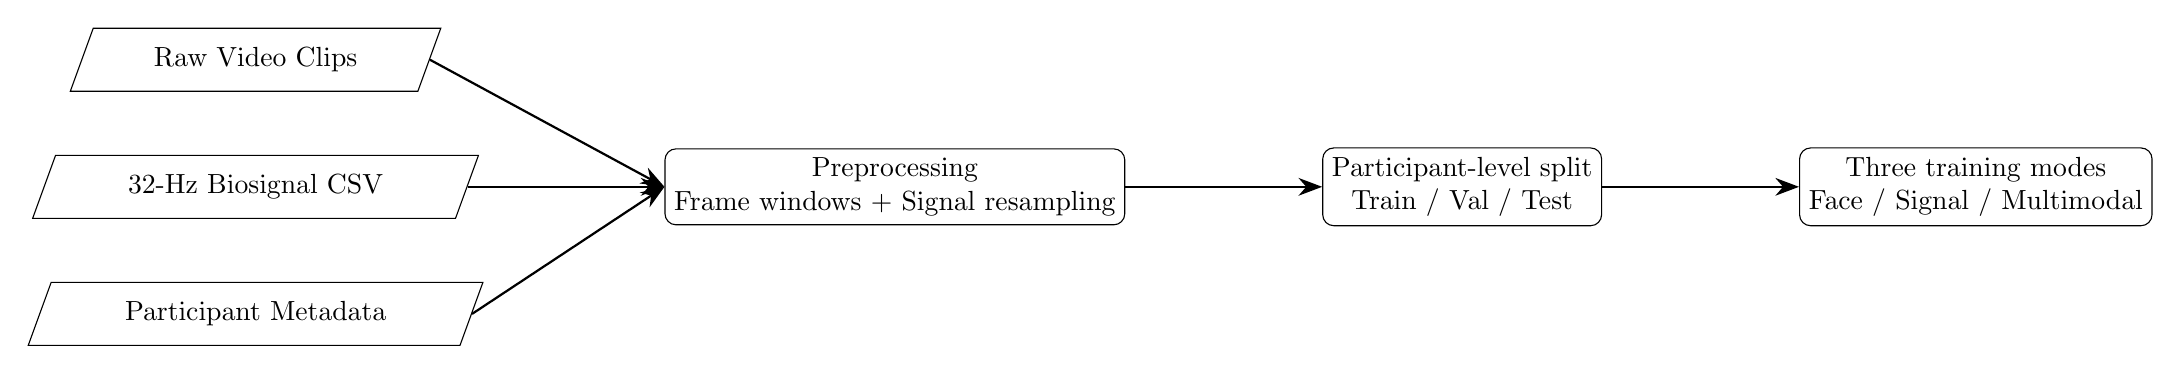
\begin{tikzpicture}[
    node distance=8mm and 10mm,
    block/.style={rectangle, rounded corners, draw=black, minimum width=3.2cm, minimum height=8mm, align=center},
    io/.style={trapezium, trapezium left angle=70, trapezium right angle=110, draw=black, minimum width=3.4cm, minimum height=8mm, align=center},
    arr/.style={-{Stealth[length=3mm]}, thick}
]
\node[io] (video) {Raw Video Clips};
\node[io, below=of video] (signal) {32-Hz Biosignal CSV};
\node[io, below=of signal] (meta) {Participant Metadata};

\node[block, right=25mm of signal] (prep) {Preprocessing\\Frame windows + Signal resampling};
\node[block, right=25mm of prep] (split) {Participant-level split\\Train / Val / Test};
\node[block, right=25mm of split] (train) {Three training modes\\Face / Signal / Multimodal};

\draw[arr] (video.east) -- (prep.west);
\draw[arr] (signal.east) -- (prep.west);
\draw[arr] (meta.east) -- (prep.west);
\draw[arr] (prep.east) -- (split.west);
\draw[arr] (split.east) -- (train.west);
\end{tikzpicture}
\end{center}

\section*{4. Model Architecture Diagram}
\begin{center}
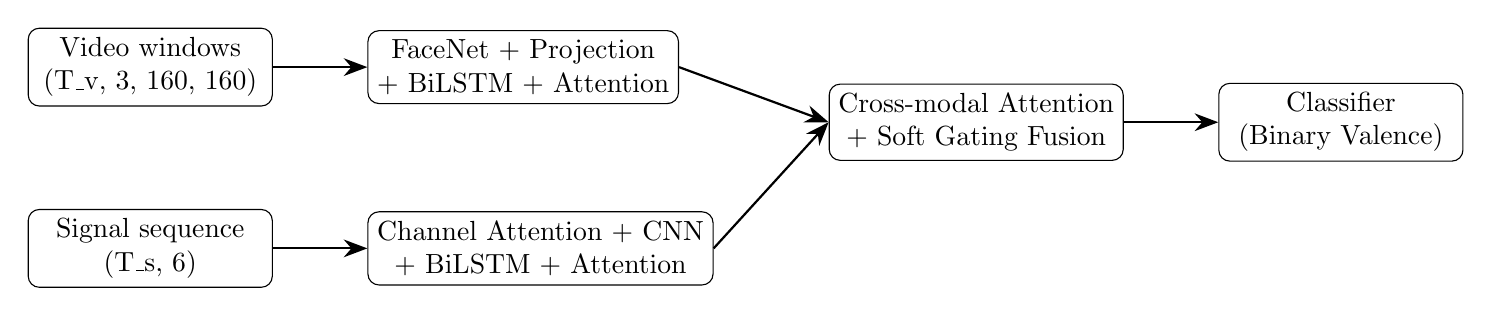
\begin{tikzpicture}[
    node distance=9mm and 12mm,
    block/.style={rectangle, rounded corners, draw=black, minimum width=3.1cm, minimum height=8mm, align=center},
    arr/.style={-{Stealth[length=3mm]}, thick}
]
\node[block] (v0) {Video windows\\(T\_v, 3, 160, 160)};
\node[block, right=of v0] (v1) {FaceNet + Projection\\+ BiLSTM + Attention};
\node[block, below=13mm of v0] (s0) {Signal sequence\\(T\_s, 6)};
\node[block, right=of s0] (s1) {Channel Attention + CNN\\+ BiLSTM + Attention};
\node[block, right=19mm of v1, yshift=-7mm] (fuse) {Cross-modal Attention\\+ Soft Gating Fusion};
\node[block, right=of fuse] (clf) {Classifier\\(Binary Valence)};

\draw[arr] (v0.east) -- (v1.west);
\draw[arr] (s0.east) -- (s1.west);
\draw[arr] (v1.east) -- (fuse.west);
\draw[arr] (s1.east) -- (fuse.west);
\draw[arr] (fuse.east) -- (clf.west);
\end{tikzpicture}
\end{center}

\section*{5. Data Augmentation and Training Policy}
\begin{itemize}
    \item Temporal jitter and sliding windows on video stream.
    \item Train dataset repeat expansion per epoch.
    \item WeightedRandomSampler with capped imbalance ratio.
    \item Focal loss + label smoothing.
    \item Modality ablation controls for fair baselines:
    face-only and physiological-only.
\end{itemize}

\section*{6. Final Results}
\begin{center}
\begin{tabular}{llrrrr}
\toprule
Model & Artifact & Test Acc & Macro-F1 & Best Epoch & Best Val Macro-F1 \\
\midrule
Facial Only & final\_valence\_face\_only & 0.4123 & 0.2919 & 1 & 0.2600 \\
Physiological Only & final\_valence\_signal\_only & 0.4123 & 0.2919 & 1 & 0.2600 \\
Multimodal & final\_valence\_multimodal & 0.4123 & 0.2919 & 1 & 0.2600 \\
Metadata-Assisted & final\_valence\_metadata & 0.6009 & 0.4934 & NA & NA \\
\bottomrule
\end{tabular}
\end{center}

\paragraph{Summary.} Best current model by macro-F1: Metadata-Assisted (macro-F1=0.4934, acc=0.6009).

\section*{7. Discussion}
Current performance is constrained mainly by weak cross-modal alignment when strict participant-ad-time keys are unavailable in processed biosignal files.
This can make multimodal training collapse toward one dominant class.

\section*{8. Conclusion}
This submission includes a complete end-to-end pipeline (facial-only, physiological-only, multimodal, metadata-assisted), data augmentation controls,
and reproducible scripts for training and report generation suitable for project evaluation.

\end{document}
